%\VignetteIndexEntry{introduction}
\documentclass{article}

%%% latex packages
\usepackage{hyperref}
\usepackage[utf8]{inputenc}
\usepackage[usenames,dvipsnames]{xcolor}

\usepackage{lipsum} % for dummy text only

%% change margins to 1" all the way around
\oddsidemargin 0.0in
\evensidemargin 0.0in
\textwidth 6.5in
\headheight 0.0in 
\topmargin 0.0in
\textheight 9.0in

%%% document info
\title{Introduction to \texttt{SpaDES}}

\author{
  Alex M. Chubaty\\
	\small{Natural Resources Canada, Pacific Forestry Centre}\\
	\small{email: \href{mailto:achubaty@nrcan.gc.ca}{achubaty@nrcan.gc.ca}}
	\and
	Eliot McIntire\\
	\small{Natural Resources Canada, Pacific Forestry Centre}\\
	\small{email: \href{mailto:emcintir@nrcan.gc.ca}{emcintir@nrcan.gc.ca}}
}

\usepackage{Sweave}
\begin{document}
\Sconcordance{concordance:introduction.tex:introduction.Rnw:%
1 31 1 1 0 14 1 1 3 2 0 1 1 1 10 8 0 1 2 7 0 1 5 14 1 1 2 1 0 4 1 1 2 4 %
0 1 2 22 1 1 2 1 0 1 4 2 0 1 2 1 0 3 1 1 5 3 0 1 1 1 2 11 0 1 1 15 0 1 %
7 5 0 1 2 5 0 1 2 7 1}

 % displays code as entered (no arranging lines)

\maketitle

\tableofcontents

\newpage

\section{Spatial Discrete Event Simulation (SpaDES)}

\paragraph{Requirements}
This packages makes heavy use of the \texttt{raster} and \texttt{sp} packages, so familiarity with these packages and their classes and methods is recommended.

\begin{Schunk}
\begin{Sinput}
> ## for now only while testing, etc.
> OS <- tolower(Sys.info()["sysname"])
> hostname <- gsub(Sys.info()["nodename"],pattern=".-VIC-",replace="")
> if (OS=="windows") {
+     if(any(pmatch(c("A105200","A105192"), hostname, nomatch=FALSE))) {
+         path <- "c:/Eliot/GitHub"
+     } else {
+         path <- "~/GitHub"
+     }
+ } else {
+     path <- "~/Documents/GitHub"
+ }
> #devtools::dev_mode(TRUE)
> devtools::load_all(file.path(path, "SpaDES")) # for development/testing
\end{Sinput}
\begin{Soutput}
Note: no visible binding for global variable 'to' 
Note: no visible global function definition for 'J' 
Note: no visible binding for global variable 'to' 
Note: no visible binding for global variable 'to' 
Note: no visible binding for global variable 'to' 
\end{Soutput}
\begin{Sinput}
> 
> ## 
> #library(SpaDES)
\end{Sinput}
\end{Schunk}


\newpage

\section{SpaDES modules}

\lipsum

\newpage

\section{Working with maps}

\paragraph{A raster map}
Sample map of habitat quality.

\begin{Schunk}
\begin{Sinput}
> # Give dimensions of dummy raster
> nx = 1.3e2
> ny = 1e2
> template = raster(nrows=ny, ncols=nx, xmn=-nx/2, xmx=nx/2, ymn =-ny/2, ymx=ny/2)
> # Make dummy maps for testing of models
> DEM = round(GaussMap(template, scale = 300, var = 0.03, speedup=1), 1)*1000
> Age = round(GaussMap(template, scale = 10, var = 0.1, speedup=1), 1)*20
> Forest_Cover = round(GaussMap(template, scale = 50, var = 1, speedup=1),2)*10
> Pct_Pine = round(GaussMap(template, scale = 50, var = 1, speedup=1),1)
> # Scale them as needed
> Age = Age/maxValue(Age)*100
> Pct_Pine = Pct_Pine/maxValue(Pct_Pine)*100
> # Make layers that are derived from other layers
> HabitatQuality = (DEM+10 + (Forest_Cover+5)*10)/100 
> HabitatQuality = HabitatQuality/maxValue(HabitatQuality)  
> # Stack them into a single stack for plotting
> habitat = stack(list(DEM,Age,Forest_Cover,HabitatQuality,Pct_Pine))
> names(habitat) = c("DEM","Age", "Forest_Cover", "HabitatQuality", "Pct_Pin")
> library(RColorBrewer)
> cols = list(
+   transparent.red=c("#00000000",paste(brewer.pal(8,"Greys"),"66",sep="")[8:1]),
+   grey = brewer.pal(9,"Greys"),
+   spectral = brewer.pal(8,"Spectral"),
+   terrain = rev(terrain.colors(100)),
+   heat = heat.colors(10),
+   topo = topo.colors(10)
+   )
> dev(4);simPlot(habitat,col = cols[c(2:5,3)])
\end{Sinput}
\end{Schunk}
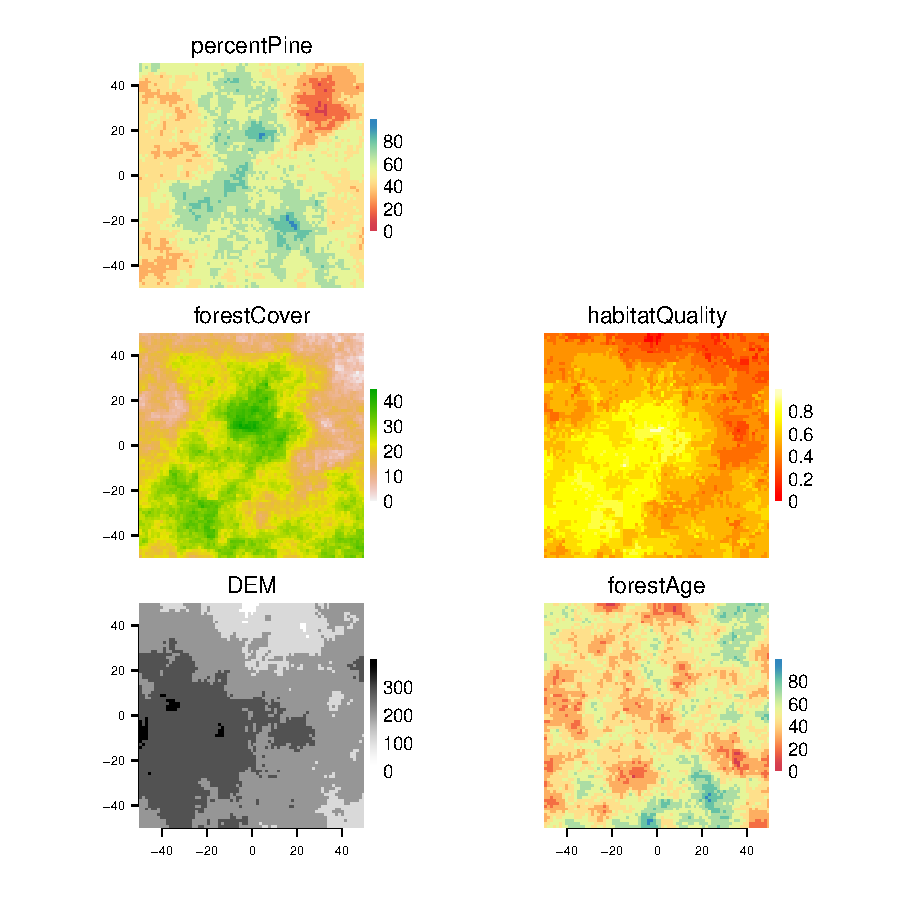
\includegraphics{introduction-habitat-map}

\newpage

\section{Simulating ``agents''}

\paragraph{}

\subsection{Spatial agents}

\subsubsection{Point agents}

\paragraph{}
Agents represented by a single set of coordinates indicating their current position.

\paragraph{}
Use a \texttt{SpatialPointsDataFrame} with additional columns as needed.

\paragraph{Non-mobile point agents}
e.g., plants

\paragraph{Mobile point agents}
e.g., animals use a \texttt{SpatialPointsDataFrame}, with additonal columns for agents' previous \texttt{n} positions, and any other columns such as age, sex, group membership, etc.

\begin{Schunk}
\begin{Sinput}
> N <- 1e1 # number of agents
> # caribou data vectors
> IDs <- c("Alice", "Bob", "Clark", "Daisy", "Eric",
+          "Franz", "Gabby", "Hayley", "Igor", "Jane")
> sex <- c("female", "male", "male", "female", "male",
+          "male", "female", "female", "male", "female")
> age <- round(rnorm(N, mean=8, sd=3))
> prevX <- runif(N, xmin(habitat)+(ncol(habitat)*0.2), xmax(habitat)-(ncol(habitat)*0.2)) # previous X location
> prevY <- runif(N, ymin(habitat)+(nrow(habitat)*0.2), ymax(habitat)-(nrow(habitat)*0.2)) # previous Y location
> # create the caribou agent object
> caribou <- SpatialPointsDataFrame(coords=cbind(x=rnorm(N, prevX, ncol(habitat)/20),
+                                                y=rnorm(N, prevY, ncol(habitat)/20)),
+                                   data=data.frame(prevX, prevY, sex, age))
> row.names(caribou) <- IDs # alternatively, add IDs as column in data.frame above
> heading(SpatialPoints(cbind(x=prevX,y=prevY)),caribou)
\end{Sinput}
\begin{Soutput}
    Alice       Bob     Clark     Daisy      Eric     Franz     Gabby    Hayley 
144.55398 182.42939  48.59348  57.57656 279.25616 171.04977 253.22975 247.84398 
     Igor      Jane 
350.33210 149.47044 
\end{Soutput}
\begin{Sinput}
> coordinates(caribou)
\end{Sinput}
\begin{Soutput}
                x          y
Alice  -30.230719 -16.677306
Bob    -10.755234 -16.146952
Clark    9.657445  13.495304
Daisy   11.463725  13.919743
Eric   -12.790430  -1.629268
Franz   23.505723 -18.996257
Gabby  -13.174640 -19.172969
Hayley  22.606989  18.325854
Igor    14.912511  24.787351
Jane   -24.689211   6.129674
\end{Soutput}
\begin{Sinput}
> ## conventional plotting method - agents don't plot properly when it is a raster stack
> #plot(habitat)
> #plot(caribou, add=TRUE)
> 
> # convenient plotting using simPlot
> simPlot(habitat,col = cols[c(2:5,3)])
> simPlot(caribou,on.which.to.plot=c(2,3,5),pch=19,size=unit(0.1,"inches"))
> drawArrows(from = SpatialPoints(cbind(x=prevX,y=prevY)),
+            to = caribou,
+            on.which.to.plot = "DEM")
\end{Sinput}
\end{Schunk}
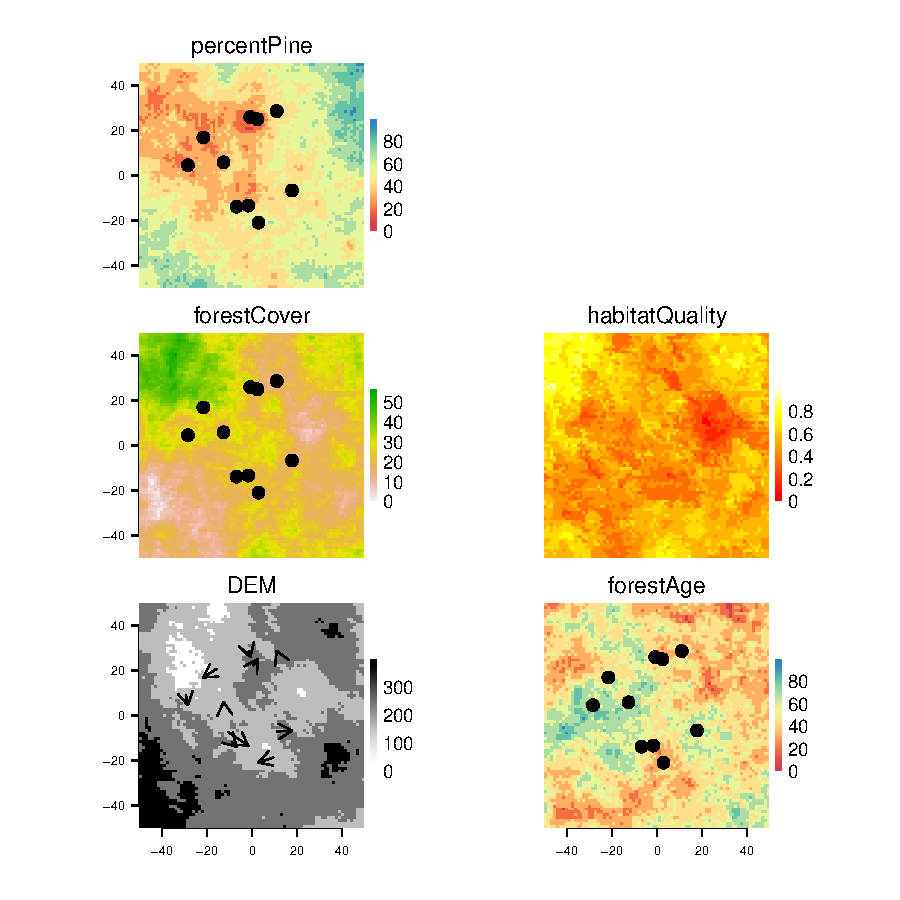
\includegraphics{introduction-mobile-point-agent}

\section{A simple fire model}
\paragraph{Burn some of the forest}
Using the spread function, we can simulate fires, and subsequent changes to the various map layers. Here, spreadProb can be a single probability or a raster map where each pixel has a probability. In the example below, each cell's probability is taken from the Percent Pine map layer.


\begin{Schunk}
\begin{Sinput}
> nFires <- 10 # number of agents
> habitat[["Fires"]] <- spread(habitat[[1]],loci=as.integer(sample(1:ncell(habitat),nFires)),
+                              spreadProb = .225,#habitat[["Pct_Pin"]]/(maxValue(habitat[["Pct_Pin"]])*5)+0.1,
+                              persistance=0,
+                              mapFireID=T,
+                              mask = NULL,
+                              maxSize = 1e8,
+                              directions = 8,
+                              iterations=1e6,
+                              plot.it=F,
+                              mapID=T)
> simPlot(habitat[["Fires"]])
\end{Sinput}
\end{Schunk}

\paragraph{}


\begin{Schunk}
\begin{Sinput}
> # Show the burning more strongly over abundant pine
> simPlot(habitat[["Pct_Pin"]],col=cols[[3]])
> simPlot(habitat[["Fires"]],add=T,delete.previous=F,col=cols[[1]])
\end{Sinput}
\end{Schunk}
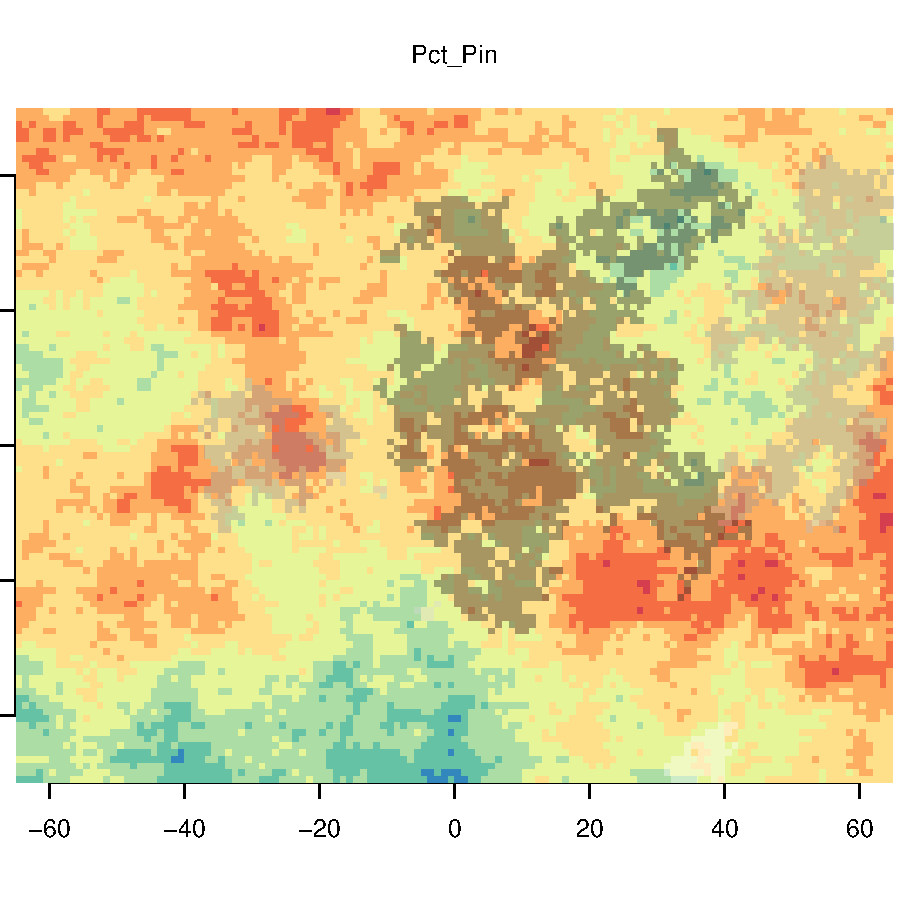
\includegraphics{introduction-fire-overlaid}


\paragraph{}
We can see that the fires tend to be in the Pines because we made it that way, using an arbitrary weighting with pine abundance

\begin{Schunk}
\begin{Sinput}
> # Show the burning more strongly over abundant pine
> fire<-reclassify(habitat[["Fires"]],rcl= cbind(0:1,c(0,ncell(habitat)),0:1))
> pine<-reclassify(habitat[["Pct_Pin"]],rcl= cbind(0:9*10,1:10*10,0:9))
> PineByFire<-crosstab(fire,pine,long=T)
> colnames(PineByFire)<-c("fire","pine","freq")
> PineByFire$pine <- as.numeric(as.character(PineByFire$pine))
> summary(glm(freq ~ fire*pine, data=PineByFire,family="poisson"))
\end{Sinput}
\begin{Soutput}
Call:
glm(formula = freq ~ fire * pine, family = "poisson", data = PineByFire)

Deviance Residuals: 
    Min       1Q   Median       3Q      Max  
-46.909  -24.265   -6.621   17.245   34.913  

Coefficients:
             Estimate Std. Error z value Pr(>|z|)    
(Intercept)  7.172729   0.017146 418.324  < 2e-16 ***
fire1       -1.379572   0.038371 -35.953  < 2e-16 ***
pine        -0.057311   0.003474 -16.495  < 2e-16 ***
fire1:pine   0.043177   0.008114   5.321 1.03e-07 ***
---
Signif. codes:  0 '***' 0.001 '**' 0.01 '*' 0.05 '.' 0.1 ' ' 1

(Dispersion parameter for poisson family taken to be 1)

    Null deviance: 14966  on 18  degrees of freedom
Residual deviance: 10937  on 15  degrees of freedom
AIC: 11082

Number of Fisher Scoring iterations: 5
\end{Soutput}
\end{Schunk}

\paragraph{}
Sure enough, there are more fires as the abundance of pine goes up, as seen by the positive interaction term (the negative fire1 term means that there are more pixels without fires than with fires).

\paragraph{Impact some of the forest}
\begin{Schunk}
\begin{Sinput}
> habitat[["Age"]][habitat[["Fires"]]>0] <- 0
> habitat[["Forest_Cover"]][habitat[["Fires"]]>0] <- 0
> habitat[["HabitatQuality"]][habitat[["Fires"]]>0] <- 0.1
> habitat[["Pct_Pin"]][habitat[["Fires"]]>0] <- 0
> simPlot(habitat,col = cols[c(2:5,3,1)])
\end{Sinput}
\end{Schunk}
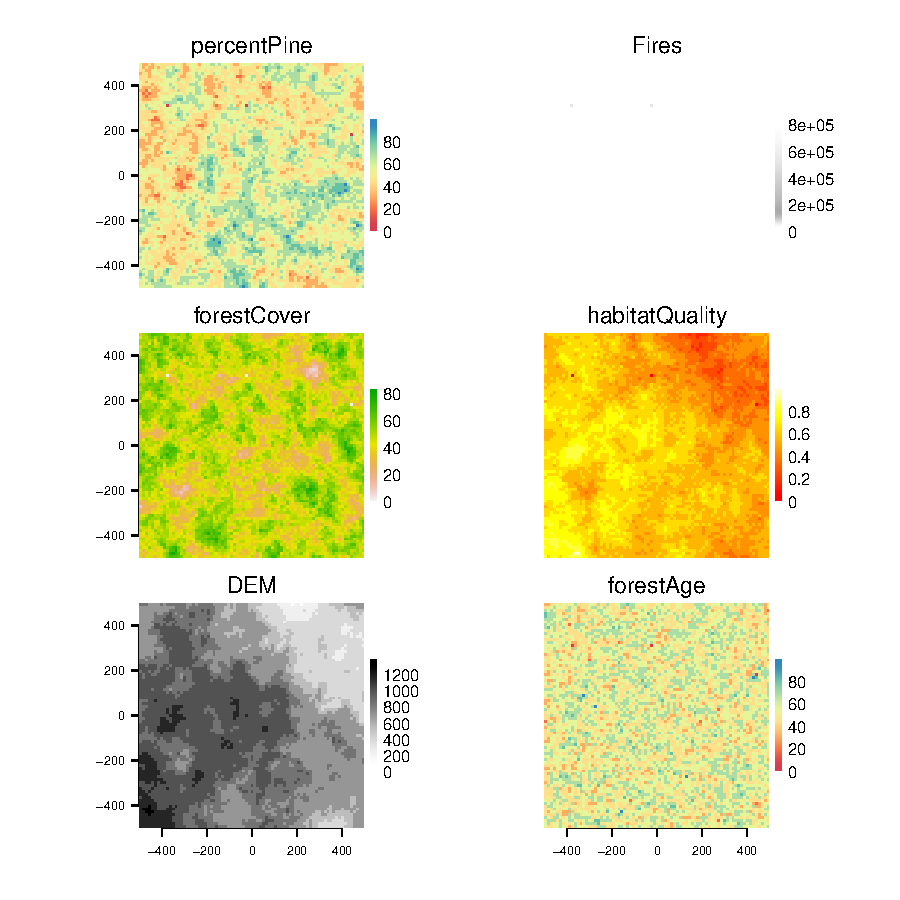
\includegraphics{introduction-Fire-impacts-maps}

\section{A simple individual based model (IBM)}
\paragraph{Move some agents}
Using a simple habitat depedent correlated random walk, simulate the movement of caribou across a heterogeneous landscape. Because we had just had fires, and we assume that fires have a detrimental effect on animal movement, we can see the long steps taken in the new, low quality, post-burn sections of the landscape.

\begin{Schunk}
\begin{Sinput}
> simPlot(habitat[["HabitatQuality"]],col = cols[[3]])
> for (i in 1:10) {
+ 
+   #crop any caribou that went off maps
+   caribou <<- crop(caribou,habitat)
+   drawArrows(from = 
+               SpatialPoints(cbind(x=caribou$prevX,y=caribou$prevY)),
+               to = caribou,length=0.04,
+               on.which.to.plot = 1)
+   
+   # find out what pixels the individuals are on now
+   ex =  habitat[["HabitatQuality"]][caribou] 
+   
+   #step length is a function of current cell's habitat quality
+   sl = 0.25/ex
+   
+   ln = rlnorm(length(ex), sl, 0.02) # log normal step length
+   sd = 30 # could be specified globally in params
+       
+   caribou <<- crw(caribou, stepLength=ln, stddev=sd, lonlat=FALSE)
+   
+ }
\end{Sinput}
\end{Schunk}
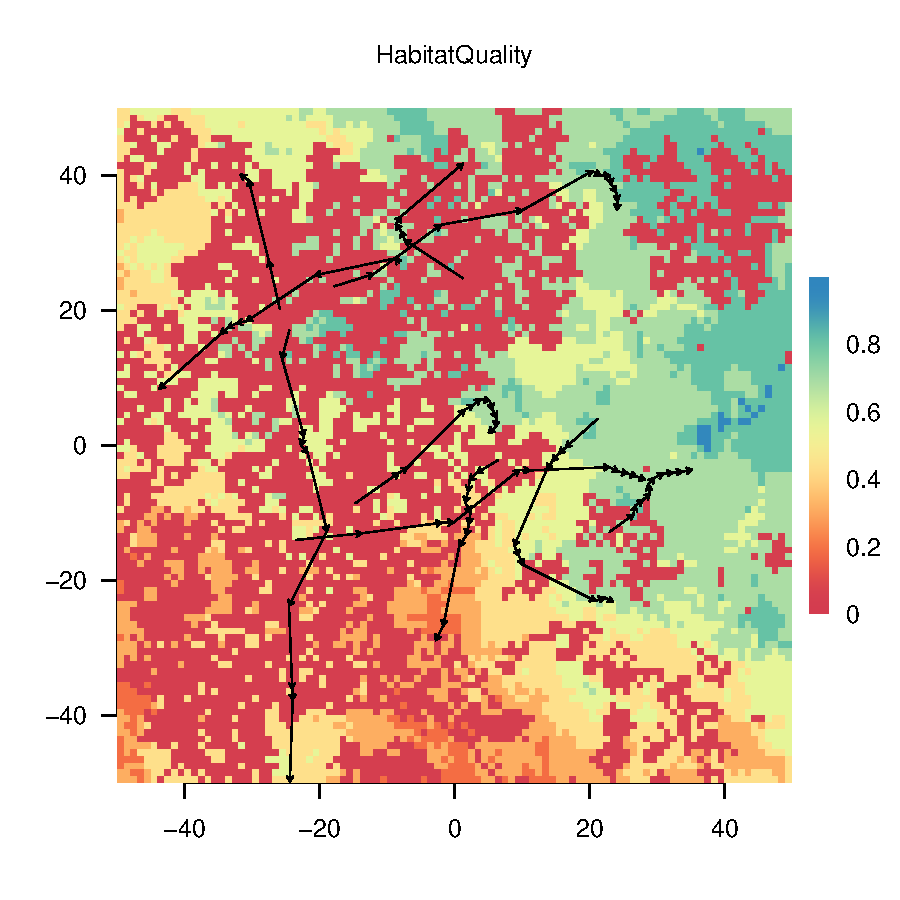
\includegraphics{introduction-Agent-crw-trajectory}

\end{document}
